% !TeX program = platex_custom
\documentclass[twocolumn,a4j]{jsarticle}
\usepackage[top=15truemm,bottom=20truemm,left=20truemm,right=20truemm]{geometry}
\usepackage{amsmath}
\usepackage{amsfonts}
\usepackage{amssymb}
\usepackage[dvipdfmx]{graphicx}
\usepackage[hang,small,bf]{caption}
\usepackage[subrefformat=parens]{subcaption}
\usepackage[dvipdfmx]{color}
\usepackage{listings}
\usepackage{listings,jvlisting}
\usepackage{framed}
\usepackage[dvipdfmx]{hyperref}
\usepackage{ascmac}
\usepackage{enumerate}
\usepackage{tabularx}
\usepackage{cancel}
\usepackage{scalefnt}
\usepackage{overcite}
\usepackage{otf}
\usepackage{multicol}
\usepackage[geometry]{ifsym}
\usepackage{array}

\renewcommand{\figurename}{Fig.}
\renewcommand{\tablename}{Table }

\lstset{
basicstyle={\ttfamily},
identifierstyle={\small},
commentstyle={\smallitshape},
keywordstyle={\small\bfseries},
ndkeywordstyle={\small},
stringstyle={\small\ttfamily},
frame={tb},
breaklines=true,
columns=[l]{fullflexible},
xrightmargin=0zw,
xleftmargin=3zw,
numberstyle={\scriptsize},
stepnumber=1,
numbersep=1zw,
lineskip=-0.5ex
}

% キャプション後ろのダブルコロンを消す
\makeatletter
\long\def\@makecaption#1#2{%
  \vskip\abovecaptionskip
  \iftdir\sbox\@tempboxa{#1\hskip1zw#2}%
    \else\sbox\@tempboxa{#1 #2}%
  \fi
  \ifdim \wd\@tempboxa >\hsize
    \iftdir #1\hskip1zw#2\relax\par
      \else #1 #2\relax\par\fi
  \else
    \global \@minipagefalse
    \hbox to\hsize{\hfil\box\@tempboxa\hfil}%
  \fi
  \vskip\belowcaptionskip}
\makeatother

% タイトル
\makeatletter
\def\@maketitle
{
\begin{center}
{\LARGE \@title \par}
\end{center}
\begin{flushright}
{\large \@date 報告書 No.40}\\
{\large M2 \@author}
\end{flushright}
\par\vskip 1.5em
}
\makeatother

\author{来代 勝胤}
\title{令和4年度 12月 第1週 報告書}
\date{2022/12/12}

\begin{document}
\columnseprule=0.1mm
\maketitle

\section*{報告内容}
\begin{enumerate}[1.]
  \item 数値シミュレーションデータの作成
  \item 撮影シミュレーションと撮影画像の作成
  \item 数値解析結果とアルゴリズム適用結果
\end{enumerate}

\section*{進捗状況}

\section{数値シミュレーションデータの作成}
粒子追跡アルゴリズムの性能評価のために,
OpenFoam による三角翼周り流れの数値解析結果から,
撮影される画像をシミュレーションによって作成する.
以下の Fig.1 に今回の数値解析に使用するモデルを示す.\\

\subsection{数値シミュレーションモデル}
\begin{figure}[htbp]
  \centering
  {
    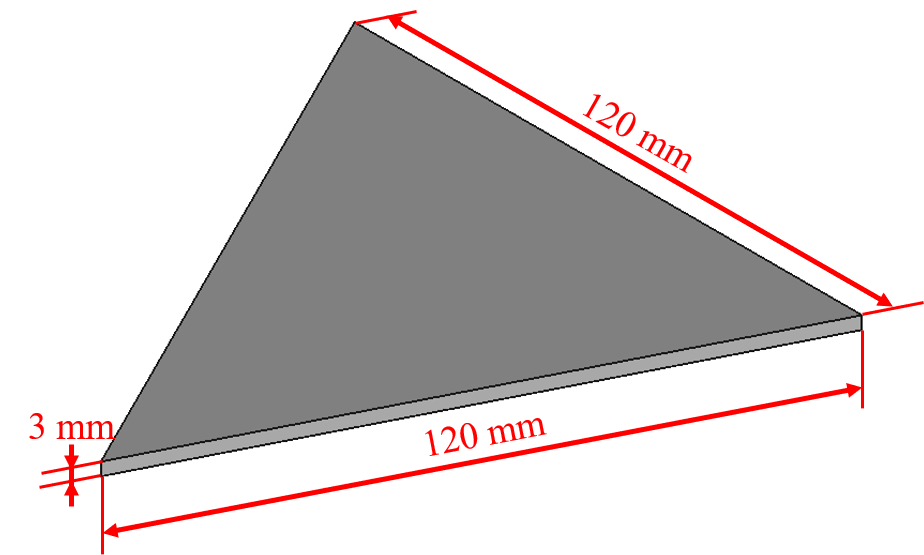
\includegraphics[keepaspectratio, width=60mm]{../images/Delta_Wing_Model.png}
    \subcaption{Delta wing Model}
    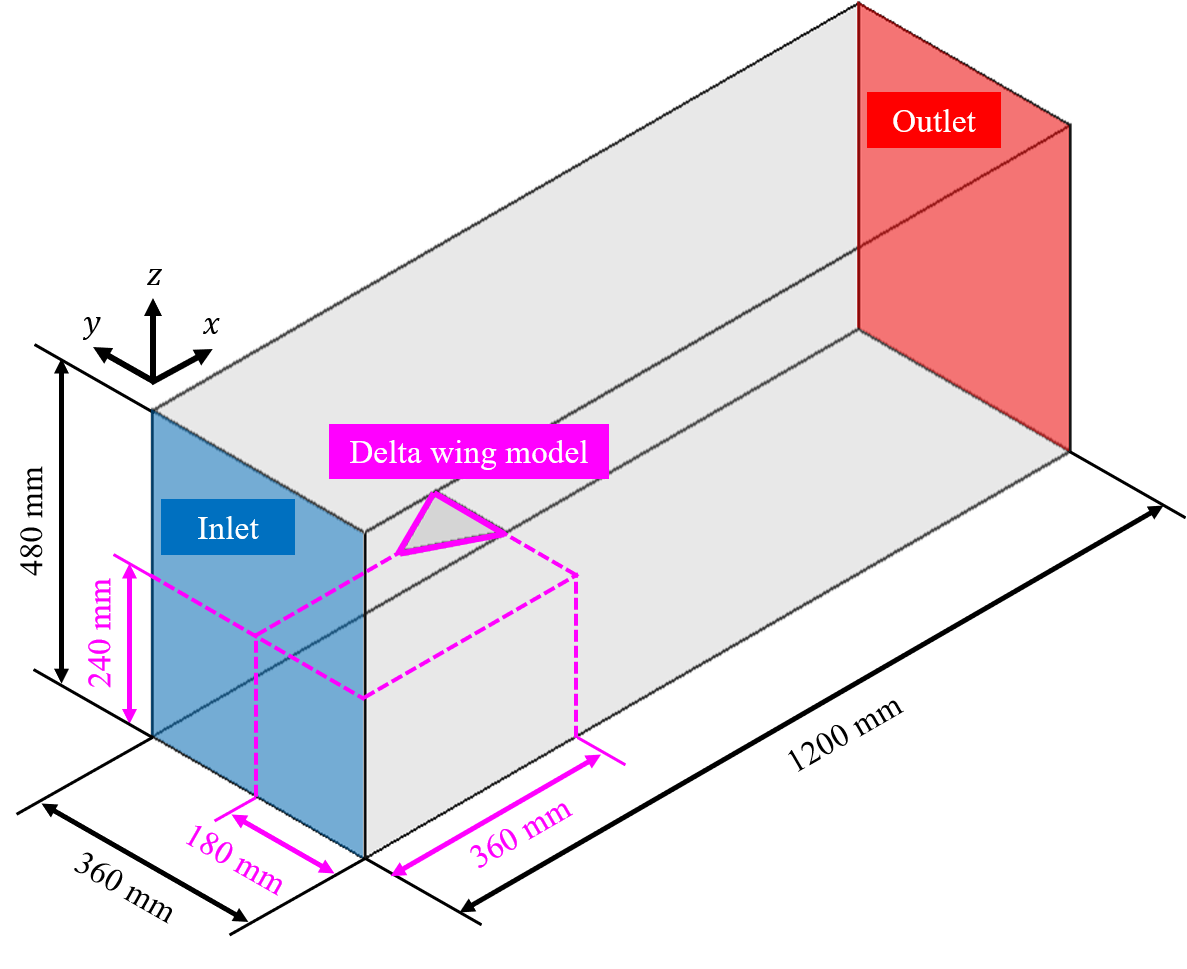
\includegraphics[keepaspectratio, width=80mm]{../images/Model_of_numerical_simulation.png}
    \subcaption{Overall view}
  }
  \caption{Numerical simulation model}
\end{figure}

\newpage

\begin{table}[hbtp]
  \centering
  \caption{Condition of numerical simulation}
  \vskip 0.2\baselineskip
  \begin{tabular}{l c c c}
    \hline
    Application           &            & OpenFOAM              \\ \hline
    Solver                &            & pimpleFoam            \\ \hline
    Turbulence model      &            & No Model              \\ \hline
    Time step             & $\Delta t$ & 1/800      & s        \\ \hline
    Simulation time       & $t$        & 5.5        & s        \\ \hline
    Characteristic length & $L$        & 120        & mm       \\ \hline
    Flow speed            & $u$        & 250        & mm/s     \\ \hline
    Kinematic viscosity   & $\nu$      & 1.004      & kg/(m·s) \\ \hline
    Reynolds number       & $\rm{Re}$  &            &          \\ \hline
  \end{tabular}\\
  \vskip 0.5\baselineskip
  ※ 初期条件は事前の数値解析結果による流れ場を利用
\end{table}

\subsection{境界条件}
\begin{table}[hbtp]
  \centering
  \caption{Boundary Conditions}
  \begin{tabular}{l c c}
           & Velocity            & Pressure     \\ \hline
    Inlet  & (-250, 0, 0) [mm/s] & zeroGradient \\ \hline
    Outlet & zeroGradient        & 0 [Pa]       \\ \hline
    Wall   & slip                & zeroGradient \\ \hline
  \end{tabular}\\
  \vskip \baselineskip
\end{table}

\section{撮影シミュレーションと撮影画像の作成}
\subsection{撮影シミュレーションのプロセス}
\begin{enumerate}[(1)]
  \item \gt{水槽座標 $(x_T, y_T, z_T)$ の計算}
  \item \gt{カメラ座標 $(x_C, y_C, z_C)$ の計算}
  \item \gt{画像座標 $(x_S, y_S, z_S)$ の計算}
  \item \gt{撮影画像の作成}
\end{enumerate}

撮影画像のシミュレーションは上記のプロセスから行われる.
はじめに,乱数で生成した粒子を数値解析から得た流れ場を利用して,
各時刻における水槽内の粒子位置(水槽座標系)を計算する.
その後,後流側から撮影することを考慮して,水槽座標系から
カメラの設置角度 $\theta$ だけ回転させたカメラ座標系を得る.
そして,カメラ座標系から撮影画像を得るために,
透視投影の原理を用いて画像座標系を計算する.
最後に,粒子の中心位置に従って
ガウス分布で輝度値を与えることによって撮影画像を作成する.

\newpage
\subsection{校正画像の生成}
撮影のシミュレーションを実行するうえで
仮想的なカメラの設置角度 $\theta$ および
カメラの設置位置の設定が非常に重要である.
パラメータの調整について,
実際の校正板の撮影画像を利用して,
それと似た画像を作成することのできる値を採用することとした.
以下の Fig.2 に実際に撮影した校正板の画像および,
撮影シミュレーションによって作成した校正板の画像を示す.

\begin{figure}[htbp]
  \centering
  \begin{tabular}{cc}
    \begin{minipage}[t]{0.45\hsize}
      \centering
      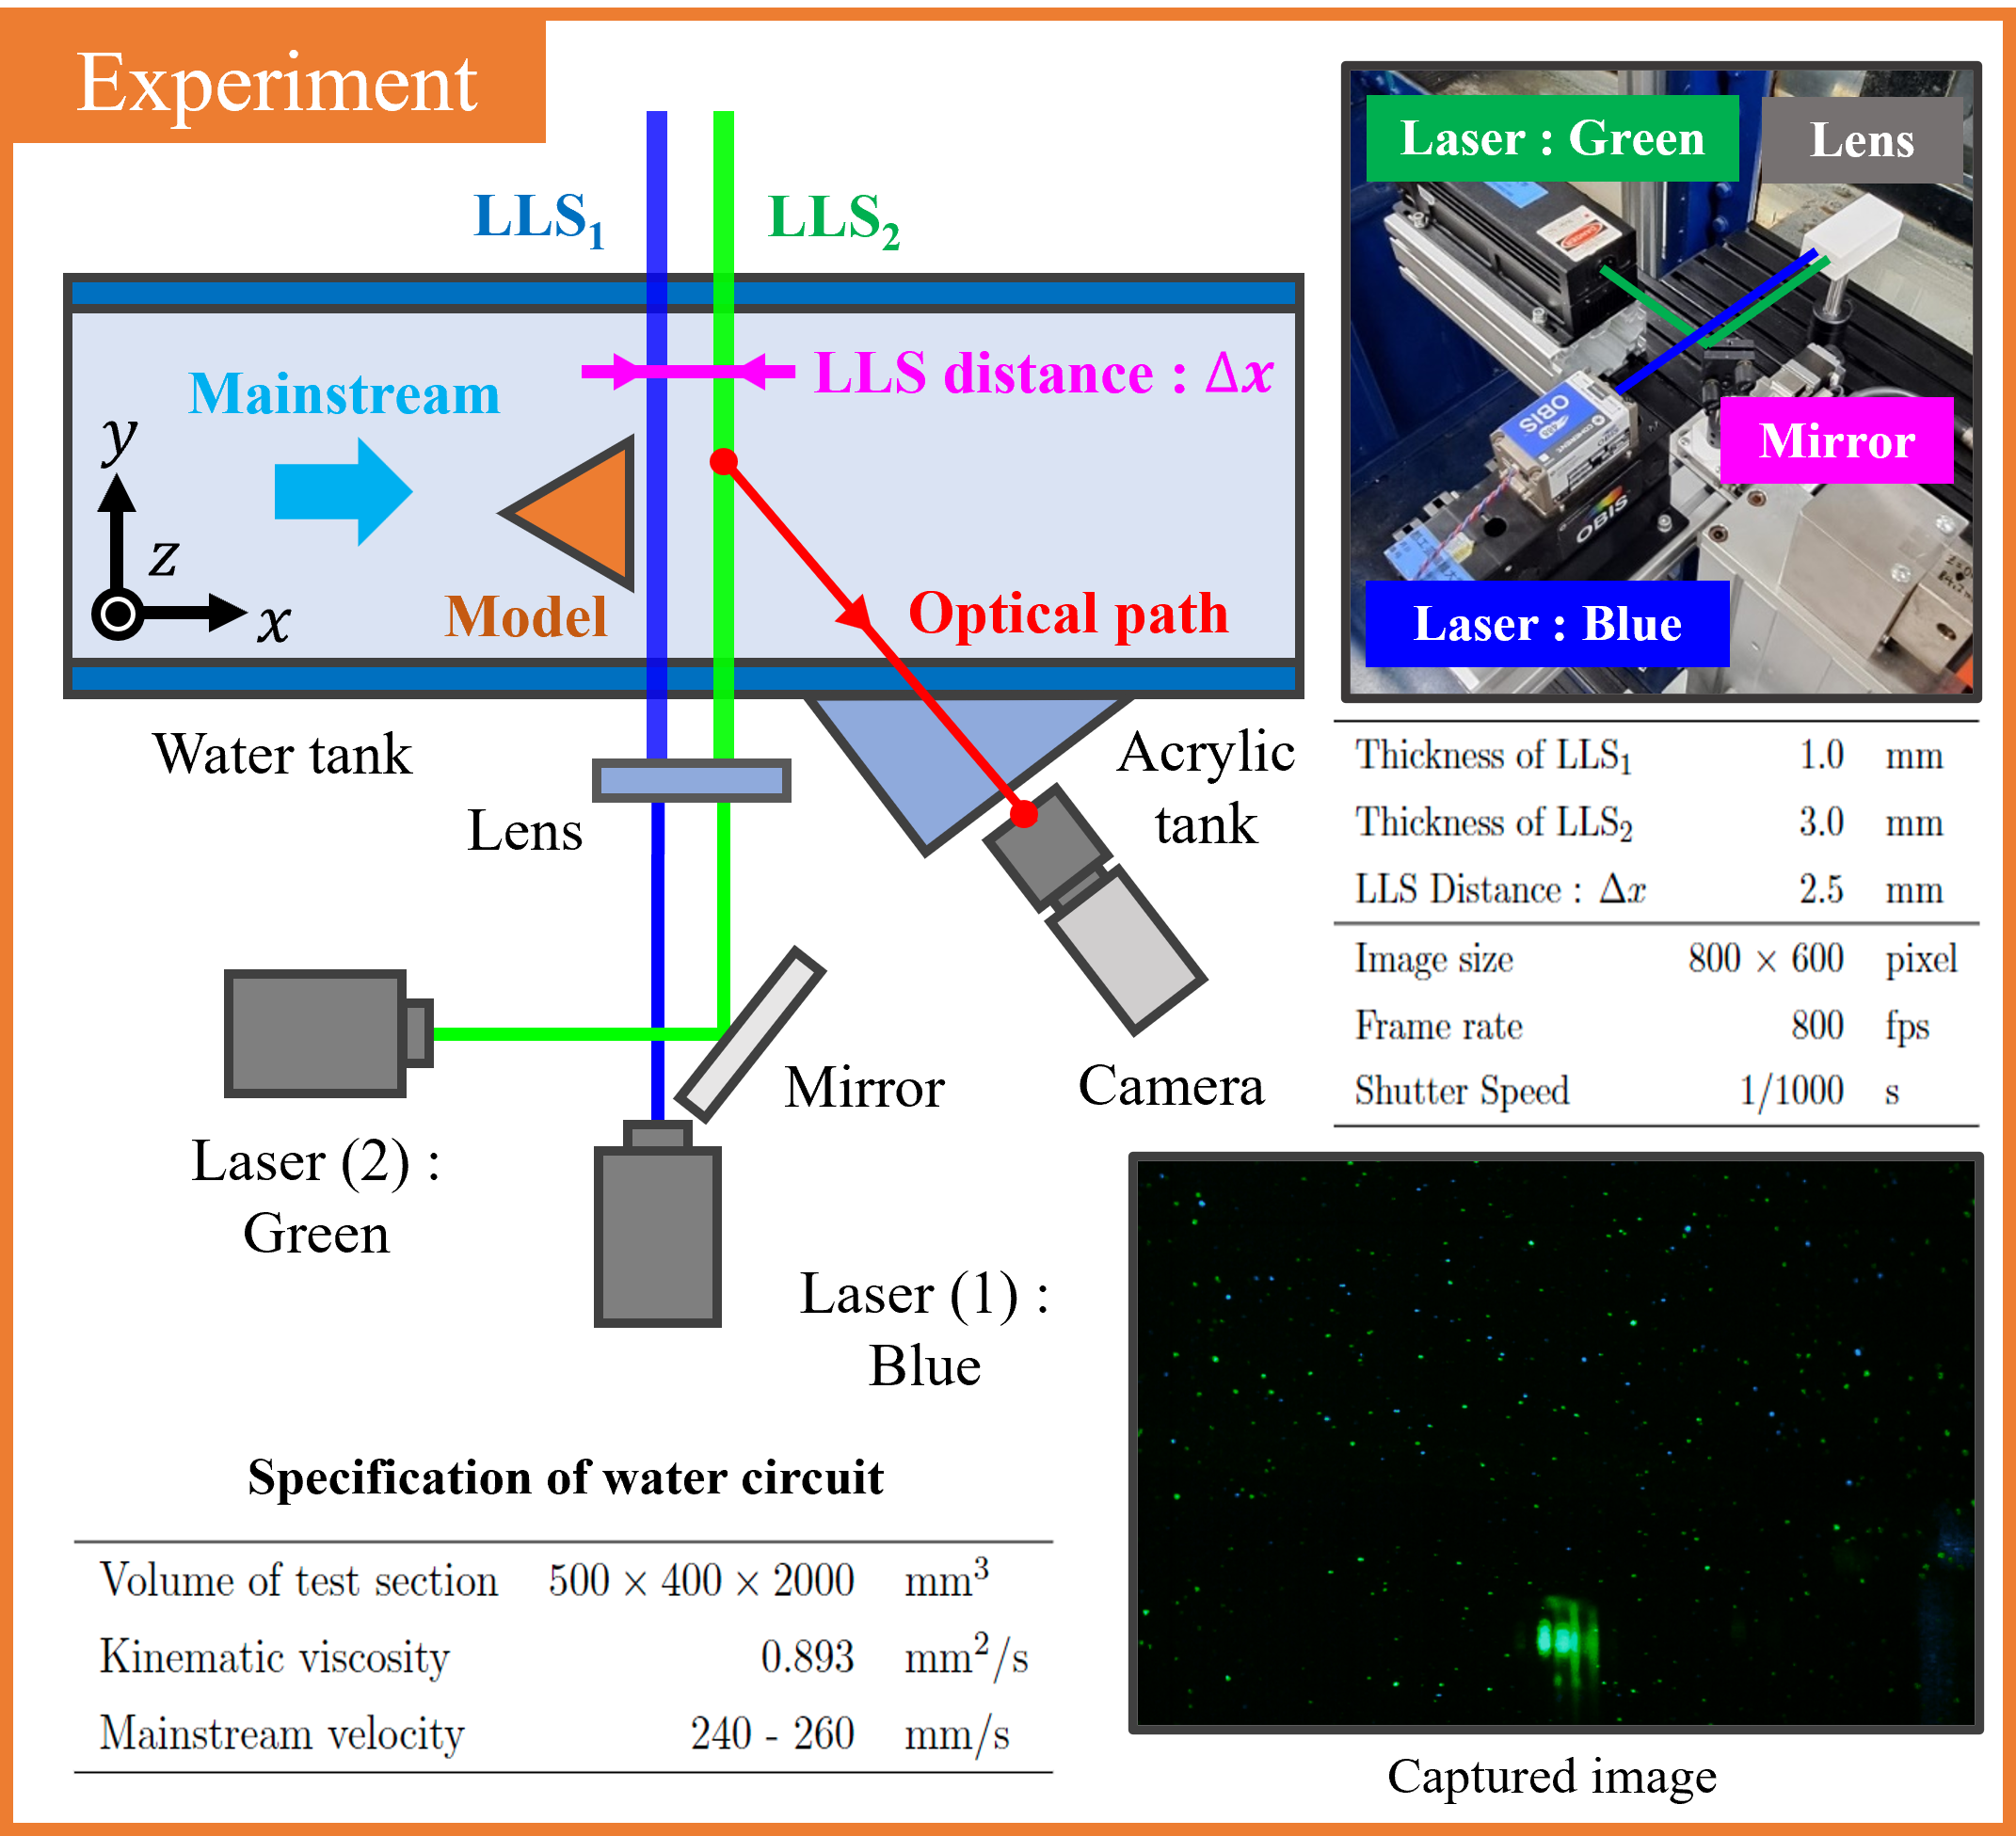
\includegraphics[keepaspectratio, width=38mm]{../images/Calibration/experiment.bmp}
      \subcaption{Experiment}
    \end{minipage} &
    \begin{minipage}[t]{0.45\hsize}
      \centering
      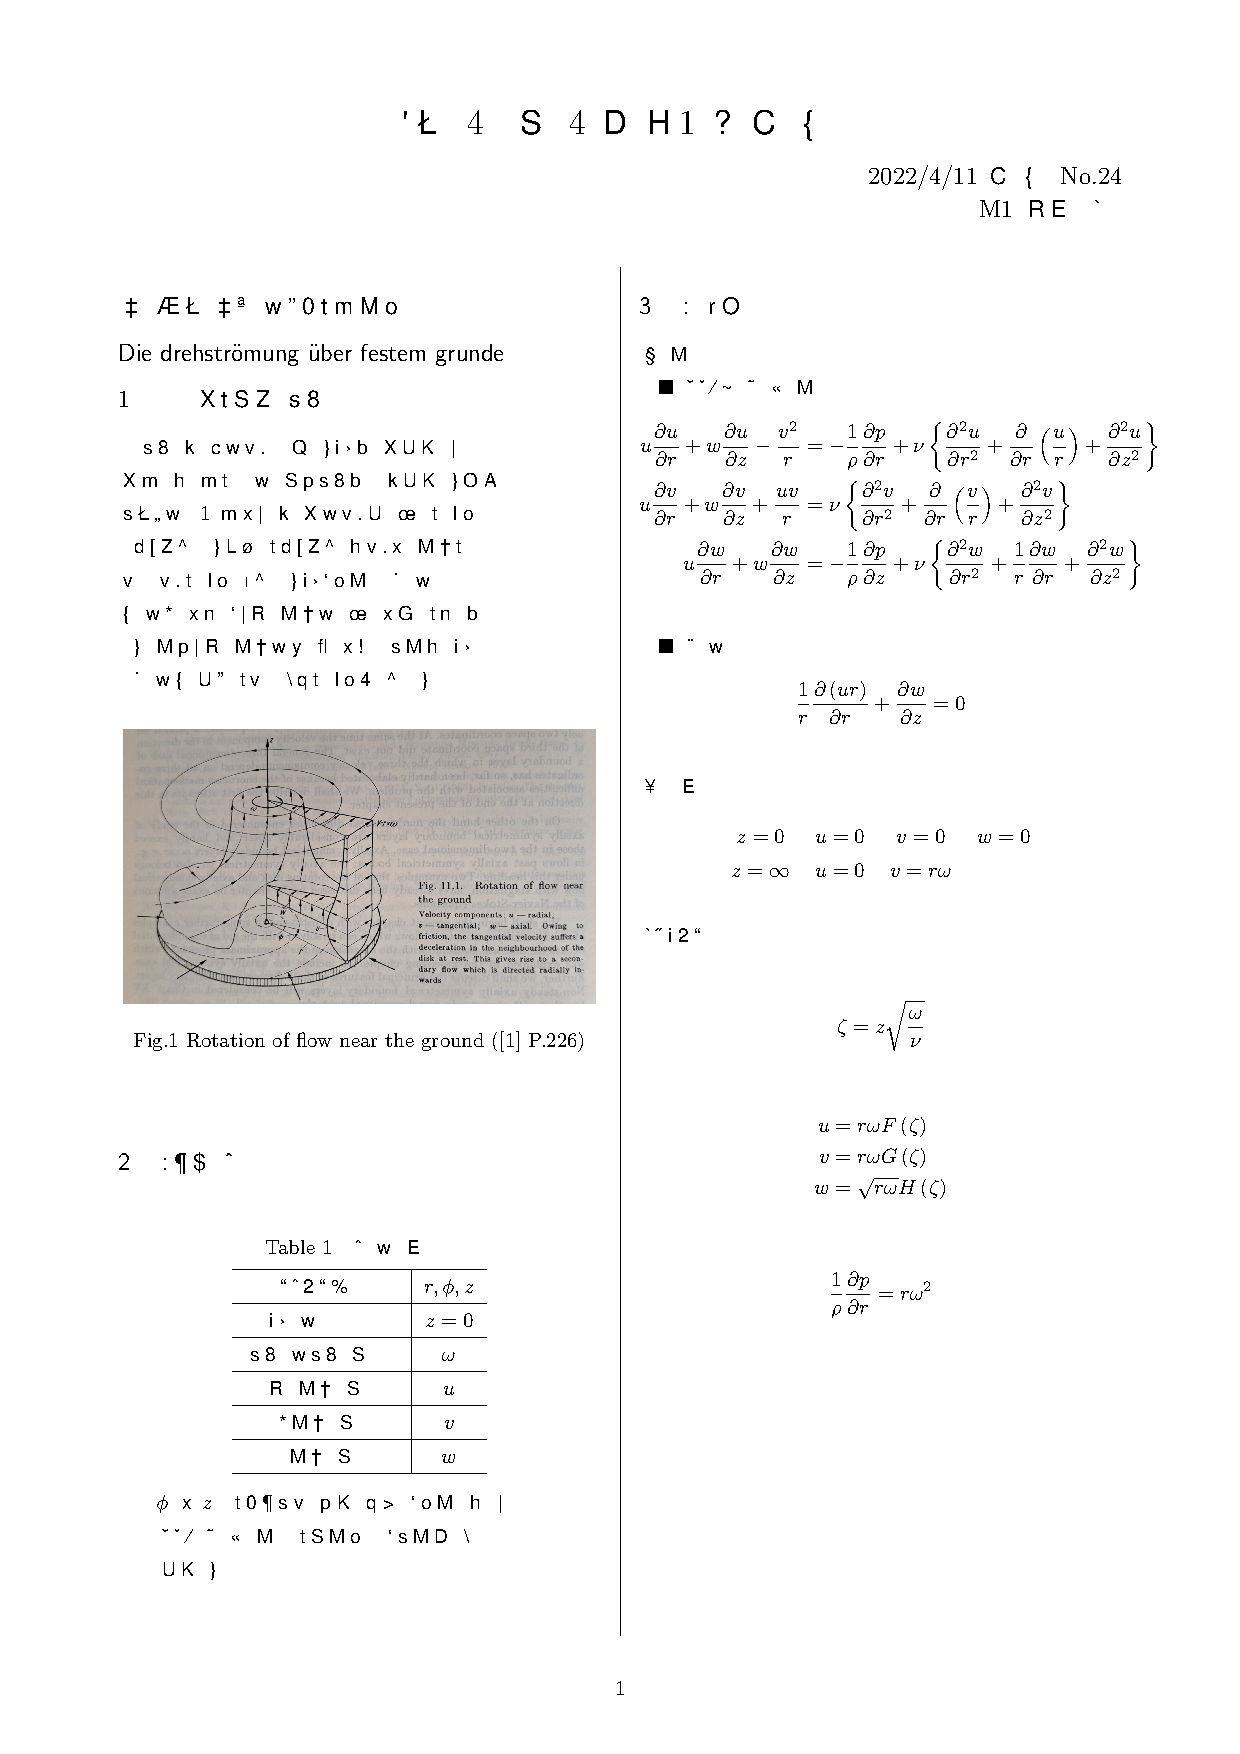
\includegraphics[keepaspectratio, width=38mm]{../images/Calibration/simulation.bmp}
      \subcaption{Numerical simulation}
    \end{minipage}
  \end{tabular}
  \caption{Image of calibration block}
\end{figure}

\section{数値解析結果とアルゴリズム適用結果}
\subsection{数値解析による流れ場}
数値解析によって取得した $x=0$ [mm] の流れ場を以下の Fig.3 に示す.
$y-z$ 平面内の速度ベクトル $(v,w)$に加えて,(a) は渦度を
(b) は 主流方向速度 $u$ を示している.
また,図内において,三角翼の後端が $x=0$ [mm],$z=20$ [mm],
三角翼の中心が $y=0$ [mm] に,右端部が $y=60$ [mm] に位置している.
結果より,三角翼の翼端部に強い渦が発生し,翼の後方の主流速度は減少していることがわかる.

\begin{figure}[htbp]
  \centering
  {
    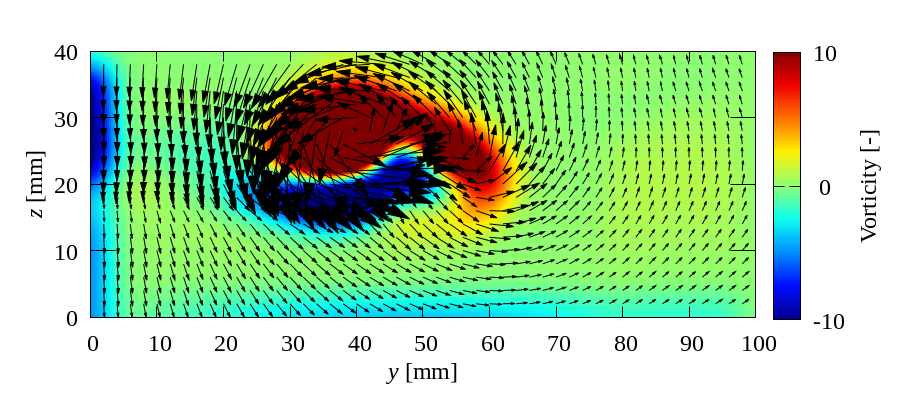
\includegraphics[keepaspectratio, width=82mm]{../images/Numerical_Simulation/velocity_and_vorticity.png}
    \subcaption{Velocity \& Vorticity}
    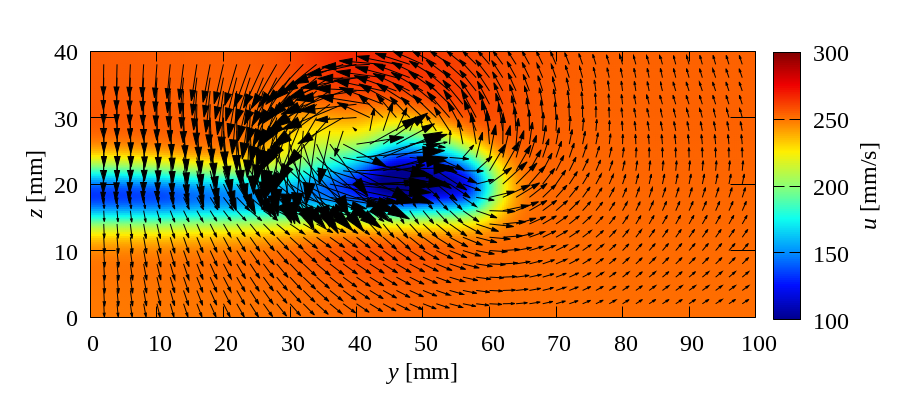
\includegraphics[keepaspectratio, width=82mm]{../images/Numerical_Simulation/velocity_xyz.png}
    \subcaption{Velocity}
  }
  \caption{Numerical simulation}
\end{figure}

\subsection{計測アルゴリズムの適用結果}
撮影シミュレーションによって作成した画像を計測アルゴリズムによって解析を行った結果を
以下の Fig.4 に示す.ここで,今回の真値となる Fig.3 の結果と比べると
大きく異なる流れ場を示していることがわかる.
特に,$y-z$ 平面内の速度ベクトルについて,
下向きの流れが誇張されて評価されている.

\begin{figure}[htbp]
  \centering
  {
    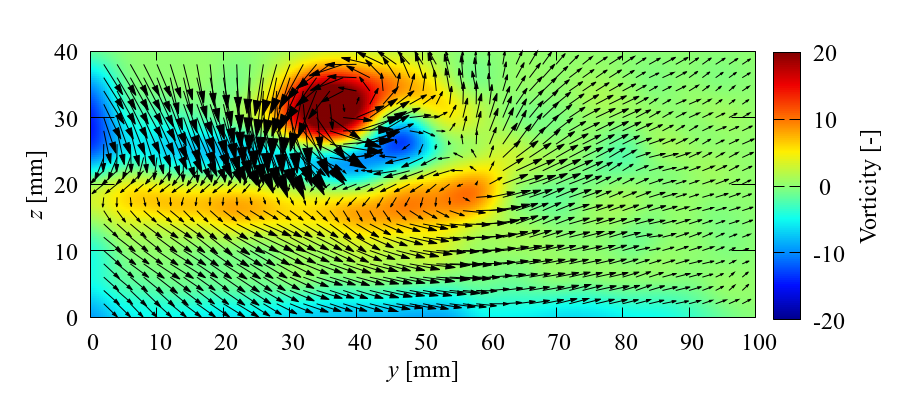
\includegraphics[keepaspectratio, width=82mm]{../images/Analysis_Result/velocity_and_vorticity.png}
    \subcaption{Velocity \& Vorticity}
    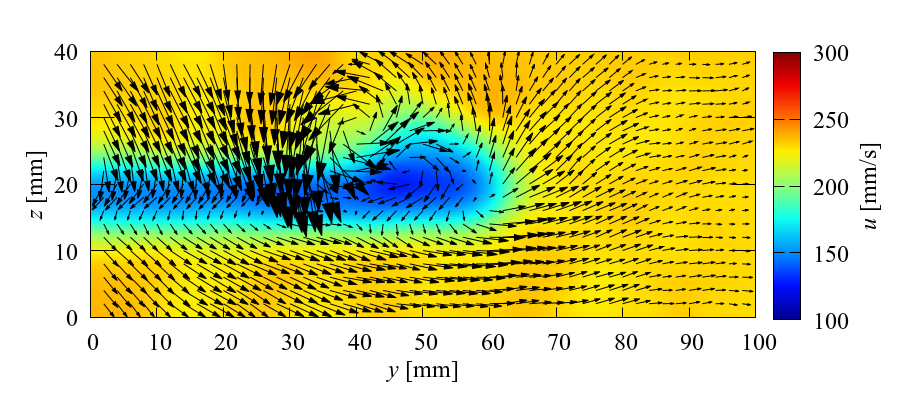
\includegraphics[keepaspectratio, width=82mm]{../images/Analysis_Result/velocity_xyz.png}
    \subcaption{Velocity}
  }
  \caption{Measurement algorithm}
\end{figure}

\subsection{実際の実験結果}
\begin{figure}[htbp]
  \centering
  {
    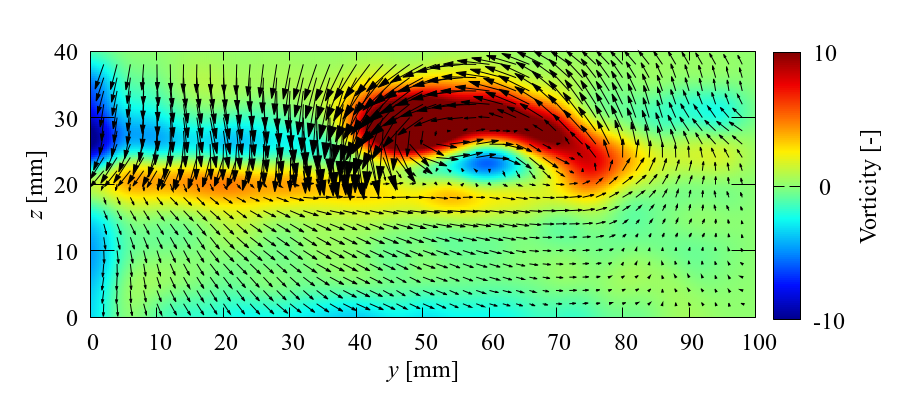
\includegraphics[keepaspectratio, width=82mm]{../images/Experiment/velocity_and_vorticity.png}
    \subcaption{Velocity \& Vorticity}
    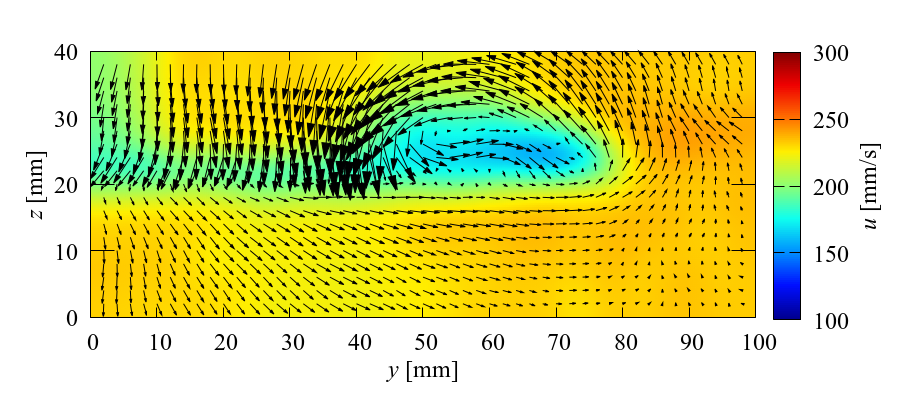
\includegraphics[keepaspectratio, width=82mm]{../images/Experiment/velocity_xyz.png}
    \subcaption{Velocity}
  }
  \caption{Experiment}
\end{figure}

\end{document}